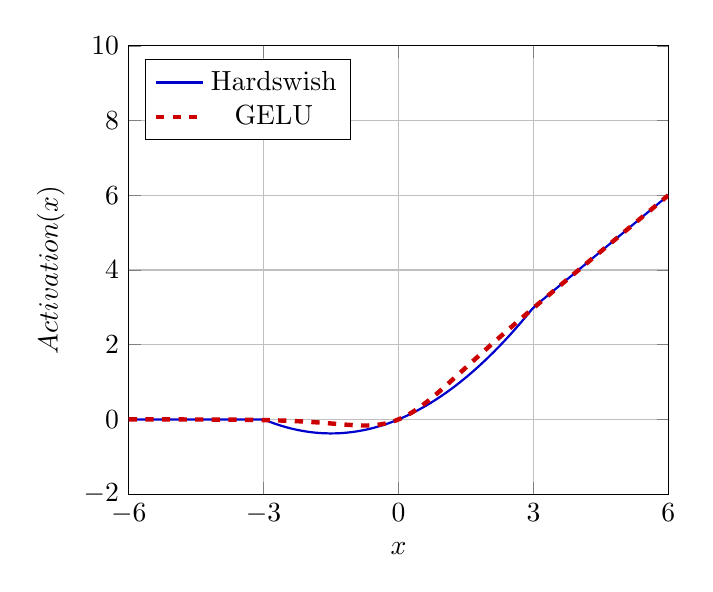
\begin{tikzpicture}
    \begin{axis}[
        grid=major,
        xlabel=$x$,
        ylabel=$\text{Activation}(x)$,
        legend pos=north west,
        xmin=-6,
        xmax=6,
        ymin=-2,
        ymax=10,
        xtick={-6,-3,...,6},
        ytick={-2,0,...,10},
    ]
        % Regular Hardswish
        \addplot[
            thick,
            color=blue!80!black,
            solid,
            samples=100,
            domain=-6:6
        ] {
            max(0,min(6,x+3)) * x / 6
        };
    
        % GELU Approximation
        \addplot[
            ultra thick,
            color=red!80!black,
            dashed,
            samples=100,
            domain=-6:6
        ] {
            x * (1 / (1 + exp(-1.702 * x)))
        };

        \legend{
            {Hardswish},
            {GELU}
        }
    \end{axis}
\end{tikzpicture}